\section{Nowcasting monthly features}
\label{chapter4_section4}


The project focuses primarily on predicting the low frequency GDP using the higher frequency information of external features. However, the prediction of these features may also represent a subject of interest on its own. A graphical representation of all the forecasts for all the features would not be manageable. A simpler alternative consists in providing a correlation matrix of the predictions generated by the models with the actual data. Figure \ref{fig_c4_s4_1} displays such a correlation matrix for the small dataset, at the nowcast horizon (one quarter ahead). In the matrix, each entry represents the correlation between a feature (columns) and its prediction (by the model given on the row). A column of high correlations (dark red entries) thus indicates a feature that is overall well predicted, whatever the model. A row of high correlations reveals a model that predicts well in general.

\begin{figure}[H]
\centering
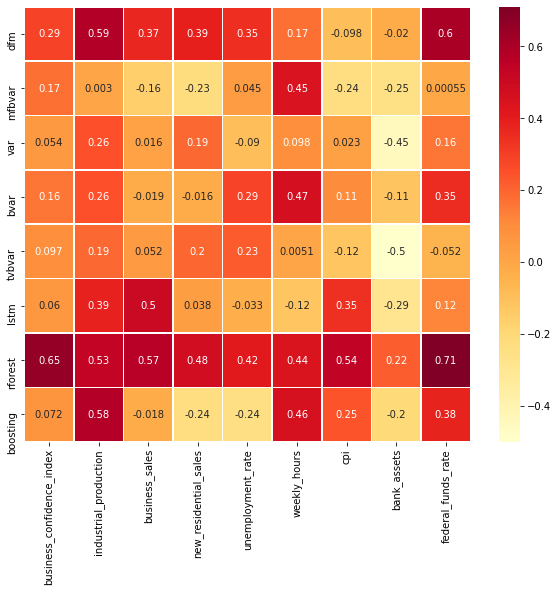
\includegraphics[scale=0.5]{images/feature_correlations.png}
\caption{Correlations: actual VS. model predictions, one quarter ahead} \vspace{-5mm}
\label{fig_c4_s4_1}
\end{figure}

\newpage

It appears that the features that are being best predicted are those strongly correlated to business cycles: industrial production, business confidence index, business sales, and weekly hours. This confirms that most of the predictive power of the models goes to business cycles related features, and thus that the models can constitute good predictors for real GDP growth rate.

Two models seem to dominate the others in tems of nowcasting: the random forest, and to a lesser extent the dynamic factor model. To confirm this intuition, a formal analysis of the RMSE errors produced by the models and benchmarks are presented in Table \ref{table_c4_s4_1}.

\begin{table}[H] \centering
\scalebox{0.6}{ \setlength{\extrarowheight}{-0.4em} \begin{tabular}{@{} llccccccccc @{}}
\toprule[0.5mm]
& & Business & Industrial & Business & New residential & Unemployment & Weekly & CPI & Bank & Federal \vspace{-2mm} \\
& & confidence index & production & sales & sales & rate & hours & & assets & Funds rate \\
\cmidrule{1-11}
\multirow{2}{*}{nowcasting} & dfm & \colorbox{coolyellow}{0,267} & \colorbox{coolgreen}{0,104} & 0,073 & 0,048 & 0,340 & 0,238 & 0,249 & 0,167 & 0,303 \\
& mfbvar & 0,341 & 0,165 & 0,099 & 0,037 & 0,398 & 0,216 & 0,322 & 0,140 & 0,252 \\
\cmidrule{1-11}
\multirow{3}{*}{econometrics} & var & 0,340 & 0,142 & 0,091 & \colorbox{coolyellow}{0,029} & 0,528 & 0,417 & 0,297 & 0,197 & 0,251 \\
& bvar & 0,311 & 0,125 & 0,078 & 0,031 & \colorbox{coolyellow}{0,309} & 0,245 & 0,249 & 0,190 & 0,216 \\
& tvbvar & 0,338 & 0,147 & 0,090 & 0,029 & 0,406 & 0,384 & 0,272 & 0,178 & 0,297 \\
\cmidrule{1-11}
\multirow{3}{*}{machine learning} & lstm & 0,320 & 0,127 & \colorbox{coolgreen}{0,056} & 0,042 & 0,462 & 0,338 & \colorbox{coolyellow}{0,211} & 0,189 & 0,265 \\
& random forest & \colorbox{coolgreen}{0,204} & \colorbox{coolyellow}{0,116} & \colorbox{coolyellow}{0,065} & \colorbox{coolgreen}{0,020} & \colorbox{coolgreen}{0,290} & \colorbox{coolgreen}{0,197} & \colorbox{coolgreen}{0,182} & \colorbox{coolgreen}{0,104} & \colorbox{coolgreen}{0,147} \\
& boosting & 0,316 & 0,126 & 0,081 & 0,035 & 0,471 & \colorbox{coolyellow}{0,210} & 0,258 & 0,190 & 0,268 \\
\cmidrule{1-11}
\multirow{2}{*}{benchmarks} & last value & 0,361 & 0,169 & 0,097 & 0,033 & 0,342 & 0,260 & 0,270 & \colorbox{coolyellow}{0,108} & \colorbox{coolyellow}{0,212} \\
& ridge var & 0,343 & 0,139 & 0,091 & 0,029 & 0,522 & 0,408 & 0,297 & 0,193 & 0,248 \\
\bottomrule[0.5mm]
\end{tabular}}
\captionsetup{justification=centering}
\caption{\textbf{Feature RMSE, 1 quarter ahead}}
\label{table_c4_s4_1}
\end{table}


The results confirm the intuition provided by the correlation matrix. The random forest represents the best model to nowcast the features in all cases, except for industrial production and business sales for which it becomes the second best. Its predictive performance is always significantly better than the competing models, with RMSE around 10-50\% smaller. 

It may look surprising that the random forest performs so well for the monthly features, while the random forest MIDAS performed only average to predict GDP. It seems that the use of the large macro dataset in the case of the random forest VAR manages to extract most of the information for feature nowcasts. By constrast, the other models, in particular in the VAR family work only on the small dataset. This may here prove insufficient as the variables in the small dataset were primarily chosen to predict GDP and may hence lack relevant information for the other features. 

\newpage

Also, the VAR models are clearly at a disadvantage since they are trained at the quarterly frequency, reducing the training sample to 1/3 of the monthly sample, and losing the underlying monthly dynamics. For the comparison to be really meaningful, the VAR models should be trained again, this time on fully monthly samples\footnote{The objective of the project consisted primarily in designing a nowcast model for GDP, which is why all the VARs were trained at the quarterly frequency. Repeating the exercise on monthly samples for the features could not be done due to lack of time}.

The other models prove hardly any better. The dynamic factor models produces decent forecasts, but constitutes the best or second best model in two cases only. The LSTM and boosting model constitute the best/second best model in only one case each. Their prediction performances are overall close to that provided by the VAR family, which supports the hypothesis that the small dataset and quarterly frequency may be at fault here.

The benchmarks, finally, look anecdotal. The last value predictor performs fair but its RMSE ar emostly above that of the other models, including the VARs. The Ridge VAR performs especially poorly.

It may also be interesting to consider the feature predictions at longer horizons. Tables \ref{table_c4_s4_2}, \ref{table_c4_s4_3} and \ref{table_c4_s4_4} display the average RMSE for the horizons of 2, 3 and 4 quarters ahead respectively.

The results are unexpected. Unlike the nowcast, the random forest almost completely disapears from the optimal models. It is replaced almost exclusively by the mixed frequency Bayesian VAR, which becomes the best model to predict at 2, 3 and 4 quarters ahead. The difference is quite significant, the mfbvar typically overperforming the random forest by about 30\%. The same conclusion stands for the other competing models. They are usually unambiguously beaten by the mfbvar, with a 10\%-30\% margin. The most serious competitor seems to be the dynamic factor model which occasionally manages to be the best or second best model, with a performance close to the mfbvar. The other models on the other hand look quite anecdotal and achieve only sub-par predictive performance.

\newpage

\begin{table}[H] \centering
\scalebox{0.6}{ \setlength{\extrarowheight}{-0.4em} \begin{tabular}{@{} llccccccccc @{}}
\toprule[0.5mm]
& & Business & Industrial & Business & New residential & Unemployment & Weekly & CPI & Bank & Federal \vspace{-2mm} \\
& & confidence index & production & sales & sales & rate & hours & & assets & Funds rate \\
\cmidrule{1-11}
\multirow{2}{*}{nowcasting} & dfm & \colorbox{coolyellow}{0,299} & \colorbox{coolyellow}{0,106} & 0,077 & 0,043 & \colorbox{coolyellow}{0,359} & 0,232 & 0,277 & 0,186 & 0,290 \\
& mfbvar & \colorbox{coolgreen}{0,244} & \colorbox{coolgreen}{0,106} & \colorbox{coolgreen}{0,043} & \colorbox{coolgreen}{0,018} & \colorbox{coolgreen}{0,229} & \colorbox{coolyellow}{0,213} & \colorbox{coolgreen}{0,163} & 0,168 & \colorbox{coolgreen}{0,165} \\
\cmidrule{1-11}
\multirow{3}{*}{econometrics} & var & 0,412 & 0,153 & 0,093 & 0,047 & 0,605 & 0,287 & 0,273 & 0,222 & 0,348 \\
& bvar & 0,309 & 0,127 & \colorbox{coolyellow}{0,060} & 0,044 & 0,443 & 0,219 & \colorbox{coolyellow}{0,232} & 0,220 & 0,307 \\
& tvbvar & 0,357 & 0,155 & 0,094 & 0,046 & 0,596 & 0,296 & 0,296 & 0,184 & 0,439 \\
\cmidrule{1-11}
\multirow{3}{*}{machine learning} & lstm & 0,332 & 0,149 & 0,064 & 0,045 & 0,447 & 0,307 & 0,238 & 0,211 & 0,286 \\
& random forest & 0,375 & 0,146 & 0,083 & \colorbox{coolyellow}{0,039} & 0,379 & 0,267 & 0,277 & \colorbox{coolgreen}{0,126} & 0,305 \\
& boosting & 0,340 & 0,139 & 0,086 & 0,041 & 0,511 & \colorbox{coolgreen}{0,210} & 0,246 & 0,261 & \colorbox{coolyellow}{0,262} \\
\cmidrule{1-11}
\multirow{2}{*}{benchmarks} & last value & 0,320 & 0,175 & 0,097 & 0,050 & 0,508 & 0,299 & 0,395 & \colorbox{coolyellow}{0,140} & 0,274 \\
& ridge var & 0,393 & 0,153 & 0,090 & 0,047 & 0,587 & 0,272 & 0,271 & 0,221 & 0,347 \\
\bottomrule[0.5mm]
\end{tabular}}
\captionsetup{justification=centering}
\caption{\textbf{Feature RMSE, 2 quarters ahead}}
\label{table_c4_s4_2}
\end{table}


\begin{table}[H] \centering
\scalebox{0.6}{ \setlength{\extrarowheight}{-0.4em} \begin{tabular}{@{} llccccccccc @{}}
\toprule[0.5mm]
& & Business & Industrial & Business & New residential & Unemployment & Weekly & CPI & Bank & Federal \vspace{-2mm} \\
& & confidence index & production & sales & sales & rate & hours & & assets & Funds rate \\
\cmidrule{1-11}
\multirow{2}{*}{nowcasting} & dfm & \colorbox{coolgreen}{0,291} & \colorbox{coolyellow}{0,124} & \colorbox{coolyellow}{0,058} & 0,047 & 0,457 & 0,263 & 0,256 & 0,208 & 0,331 \\
& mfbvar & 0,305 & \colorbox{coolgreen}{0,101} & \colorbox{coolgreen}{0,050} & \colorbox{coolgreen}{0,020} & \colorbox{coolyellow}{0,374} & \colorbox{coolgreen}{0,243} & \colorbox{coolgreen}{0,203} & 0,211 & \colorbox{coolgreen}{0,140} \\
\cmidrule{1-11}
\multirow{3}{*}{econometrics} & var & 0,397 & 0,190 & 0,097 & 0,048 & 0,521 & 0,337 & 0,221 & 0,202 & 0,434  \\
& bvar & 0,354 & 0,131 & 0,069 & 0,045 & 0,401 & \colorbox{coolyellow}{0,256} & 0,222 & 0,223 & 0,355 \\
& tvbvar & 0,379 & 0,189 & 0,097 & 0,048 & 0,440 & 0,322 & \colorbox{coolyellow}{0,204} & \colorbox{coolyellow}{0,158} & 0,534 \\
\cmidrule{1-11}
\multirow{3}{*}{machine learning} & lstm & 0,347 & 0,144 & 0,060 & \colorbox{coolyellow}{0,037} & 0,404 & 0,292 & 0,234 & 0,246 & \colorbox{coolyellow}{0,234} \\
& random forest & 0,319 & 0,171 & 0,066 & 0,045 & 0,410 & 0,296 & 0,287 & \colorbox{coolgreen}{0,143} & 0,351 \\
& boosting & 0,420 & 0,164 & 0,071 & 0,042 & \colorbox{coolgreen}{0,274} & 0,301 & 0,239 & 0,225 & 0,395 \\
\cmidrule{1-11}
\multirow{2}{*}{benchmarks} & last value & \colorbox{coolyellow}{0,291} & 0,210 & 0,083 & 0,051 & 0,390 & 0,321 & 0,338 & 0,165 & 0,365 \\
& ridge var & 0,390 & 0,181 & 0,094 & 0,048 & 0,487 & 0,325 & 0,218 & 0,209 & 0,432 \\
\bottomrule[0.5mm]
\end{tabular}}
\captionsetup{justification=centering}
\caption{\textbf{Feature RMSE, 3 quarters ahead}}
\label{table_c4_s4_3}
\end{table}


\begin{table}[H] \centering
\scalebox{0.6}{ \setlength{\extrarowheight}{-0.4em} \begin{tabular}{@{} llccccccccc @{}}
\toprule[0.5mm]
& & Business & Industrial & Business & New residential & Unemployment & Weekly & CPI & Bank & Federal \vspace{-2mm} \\
& & confidence index & production & sales & sales & rate & hours & & assets & Funds rate \\
\cmidrule{1-11}
\multirow{2}{*}{nowcasting} & dfm & 0,309 & \colorbox{coolgreen}{0,117} & \colorbox{coolgreen}{0,056} & 0,051 & 0,464 & \colorbox{coolyellow}{0,245} & 0,234 & 0,210 & 0,421 \\
& mfbvar & 0,346 & \colorbox{coolyellow}{0,122} & \colorbox{coolyellow}{0,064} & \colorbox{coolgreen}{0,035} & 0,452 & \colorbox{coolgreen}{0,220} & 0,237 & 0,215 & \colorbox{coolgreen}{0,311} \\
\cmidrule{1-11}
\multirow{3}{*}{econometrics} & var & \colorbox{coolyellow}{0,304} & 0,166 & 0,065 & 0,049 & 0,478 & 0,303 & \colorbox{coolgreen}{0,179} & 0,190 & 0,427 \\
& bvar & 0,312 & 0,141 & 0,070 & 0,046 & 0,433 & 0,255 & 0,216 & 0,201 & 0,456 \\
& tvbvar & 0,361 & 0,176 & 0,082 & 0,049 & 0,445 & 0,335 & \colorbox{coolyellow}{0,183} & \colorbox{coolgreen}{0,136} & 0,485 \\
\cmidrule{1-11}
\multirow{3}{*}{machine learning} & lstm & 0,386 & 0,147 & 0,069 & \colorbox{coolyellow}{0,043} & 0,475 & 0,310 & 0,213 & 0,214 & \colorbox{coolyellow}{0,345} \\
& random forest & 0,359 & 0,181 & 0,090 & 0,043 & \colorbox{coolyellow}{0,419} & 0,310 & 0,266 & \colorbox{coolyellow}{0,141} & 0,411 \\
& boosting & 0,386 & 0,181 & 0,079 & 0,051 & \colorbox{coolgreen}{0,318} & 0,310 & 0,193 & 0,190 & 0,494 \\
\cmidrule{1-11}
\multirow{2}{*}{benchmarks} & last value & 0,441 & 0,219 & 0,107 & 0,051 & 0,496 & 0,321 & 0,299 & 0,156 & 0,424 \\
& ridge var & \colorbox{coolgreen}{0,303} & 0,158 & 0,065 & 0,050 & 0,465 & 0,288 & 0,184 & 0,198 & 0,427 \\
\bottomrule[0.5mm]
\end{tabular}}
\captionsetup{justification=centering}
\caption{\textbf{Feature RMSE, 4 quarters ahead}}
\label{table_c4_s4_4}
\end{table}


It is difficult to explain this change in performance between the random forest and the mfbvar. To clarify the case, Figure \ref{fig_c4_s4_2} plots the predictions for the radom forest and mixed frequency Bayesian VAR models at the one, two and three quarter horizon, for a selection of features exhibiting strong performance reversal between the random forest and the mfbvar.

\begin{figure}[H]
\centering
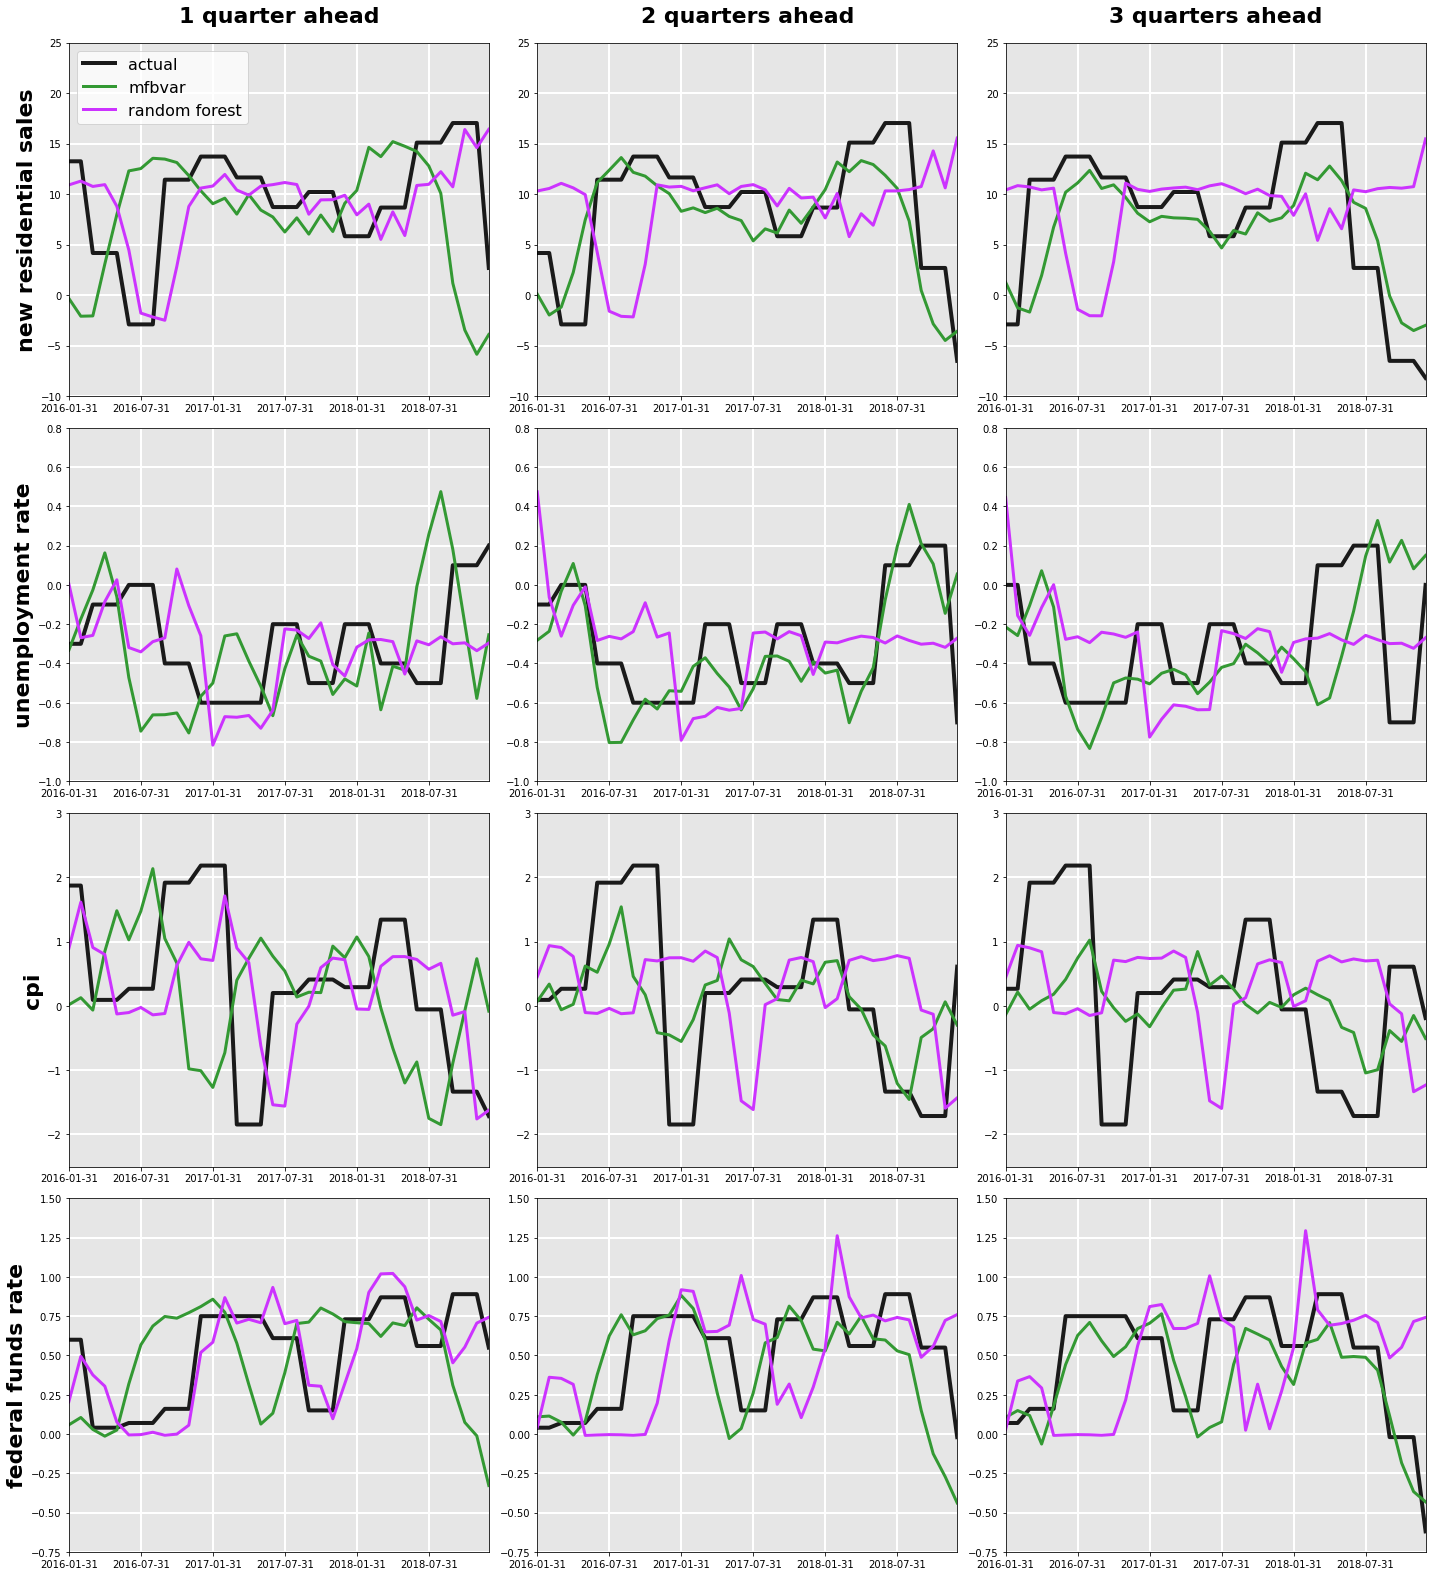
\includegraphics[scale=0.32]{images/predictions_mfbvar_rf.png}
\caption{Predictions of random forest and mixed frequency Bayesian VAR} \vspace{-5mm}
\label{fig_c4_s4_2}
\end{figure}

A pattern seems to emerge. The random forest captures the dynamics quite adequately at the nowcast horizon. Beyond the nowcast, however, it gradually starts lagging behind, which results in poor accuracy. By contrast, the mixed frequency Bayesian VAR seems to work the opposite way. As surprising at it may look, the model appears to anticipate the dynamic pattern at nowcast horizons. That is, it seems to identify correctly the overall direction of the dynamics, but somewhat too early. Following, the random forest proces more accurate for nowcasts. At the two, three and four quarters ahead horizon however, the mfbvar predictions do not precede anymore the actual movemements of the data, and become better than the laggy random forests predictions. They become, in fact, quite close to the actual dynamics.

It is quite difficult to explain this behaviour. The only difference in terms of dataset between the two models is the presence of low frequency, GDP data in the mfbvar. Possibly, this key economic variable contains forward  information on the features, which produces this anticipated behaviour. Possiby also, the Minnesota prior allows for a more easily mean-reverting model behaviour, rendering anticipations possible. Overall, these explanations are only mildly convincing, but the anticipation behaviour looks clear and unambiguous. 

At the end of the exercise, the conclusions are clear. At the nowcast horizon, the random forest dominates. The class of VAR models however should not be discared as their restricted dataset and quarterly frequency place them at a strong disadvantage. More testing is probably necessary. At longer horizons, the mixed frequency Bayesian VAR becomes optimal, as it replicates closely the actual behaviour of the data. This is in contrast with the nowcasts where it seems to anticipate the dynamics and exhibits inadequate moves.






